\documentclass[11pt, dvipsnames,aspectratio=169]{beamer}
\usetheme{Madrid}

\usepackage[utf8]{inputenc}
\usepackage{tabularray}	% for "tblr"
\usepackage{graphicx}

% Define the colors used by DNP for branding and addresses/trenches
\usepackage{xcolor}
\definecolor{dnpblue}{RGB}{0,26,174}
\definecolor{dnplightblue}{RGB}{221,226,255}
\definecolor{addressgreen}{RGB}{84,174,74}
\definecolor{addressyellow}{HTML}{ffff00}
\definecolor{addressorange}{RGB}{228,187,114}
\definecolor{addressblue}{RGB}{72,123,182}
\definecolor{addresspink}{RGB}{201,23,199}
\definecolor{addressblack}{RGB}{11,1,2}
\definecolor{trenchgreen}{HTML}{54b04a}
\definecolor{trenchred}{HTML}{db1e2a}
\definecolor{trenchblue}{HTML}{487bb6}
\definecolor{trenchlightblue}{HTML}{00b0f0}
\definecolor{trenchorange}{HTML}{ffba0b}
\definecolor{trenchpurple}{HTML}{873bde}
\definecolor{trenchspuelbohrung}{HTML}{01ffe1}
\definecolor{trenchblack}{HTML}{000000}
\colorlet{beamer@blendedblue}{dnpblue}

% define the fading used on the title slide
\usepackage{tikz}
\usetikzlibrary{fadings,calc}
\tikzfading[name=dnpfading,top color=transparent!100,bottom color=transparent!0]

\tikzset{fotopunkt/.style={scale=.7,inner sep=1pt,text=white,draw=white,fill=dnpblue,circle}}
% draw the zoom triangle between a point of interest and its photo
%  * label of the point (#1)
%  * photo (as a TikZ node) (#2)
%  * x, y coordinates of the point within the current map (#3, #4)
\newcommand\zoomtriangle[4]{
	\tikz[remember picture,overlay]{
		\coordinate (top) at ($(map.north west)!#3!(map.north east)$);
		\coordinate (bottom) at ($(map.south west)!#3!(map.south east)$);
		\coordinate (target) at ($(top)!#4!(bottom)$);
		\fill[gray,opacity=.35] (target) -- (#2.north west) -- (#2.south west) -- cycle;
		\node[fotopunkt] at (target) {#1};
	}
}

% dot to signify an address
\newcommand\colordot[1]{\tikz{\draw[white,opacity=0] (0,0) -- (0,-.12);\draw[white,opacity=0] (0,0) -- (.2,0);\node[inner sep=-2,circle,draw=black,fill=#1] at (0,0) {};}}

% short rule to signify a trench
\newcommand\colorrule[1]{\tikz{\draw[white,opacity=0] (0,0) -- (0,-.08);\draw[white,opacity=0] (0,0) -- (.58,0);\fill[#1] (0,0) rectangle (.51,.08);}}


% bulletlist is an itemized list which has a blue bullet before each item
\setbeamertemplate{itemize items}{$\bullet$}
\newenvironment{bulletlist}[1]{\begin{itemize}\setlength{\itemsep}{#1}}{\end{itemize}}

% define a new environment "mapframe" which consists of
%  * a title (#1)
%  * a left column featuring an image (#2) of width #3
%  * a right column containing the content of the environment
% example:
% \begin{mapframe}{Frame title}{/path/to/map.png}{.5\textwidth}
%     (content of the right column)
% \end{mapframe}
\usepackage{environ,calc}
\NewEnviron{mapframe}[3]{\begin{frame}{#1}
	\begin{minipage}{#3}
		\tikz[remember picture]{\node[inner sep=0] (map) at (0, 0) {\includegraphics[width=\linewidth]{#2}};}
	\end{minipage}\hfill%
	\begin{minipage}{\dimexpr0.99\linewidth-#3}\BODY\end{minipage}
\end{frame}}

% logo in the bottom right corner
\logo{
\includegraphics[width=.1\textwidth]{../Bilder/Logo.png}}
\newcommand{\nologo}{\setbeamertemplate{logo}{}} % command to set the logo to nothing

% info shown in the footline
\author{Deutsche Netzplanung}
\title{Ergebnisse \Ort}
\date{\Abgabedatum}

% No navigation symbols ("next slide"/"previous slide")
\setbeamertemplate{navigation symbols}{}

% make the footline DNP blue
\setbeamercolor{palette primary}{bg=dnpblue,fg=white}
\setbeamercolor{palette secondary}{bg=dnpblue,fg=white}
\setbeamercolor{palette tertiary}{bg=dnpblue,fg=white}

% read variable data
% Ort
\newcommand{\Ort}{TODO}

% Landkreis
\newcommand{\Kreis}{TODO}

% Bundesland
\newcommand{\Land}{TODO}

% Abgabedatum
\newcommand{\Abgabedatum}{TODO}

% Kunde, z.B. GF+ oder FED
\newcommand{\Kunde}{TODO}

% Text beim Analysebeispiel für den Adresscheck
\newcommand{\adresseAnalysebeispiel}{TODO}

% Anzahl der Einheiten im Analysebeispiel
% Format: Grunddaten GF+ & Adresscheck DNP & Differenz
% Beispiel: 39 & 36 & -3
\newcommand{\einheitenAnalysebeispiel}{TODO & TODO & TODO}

% Text bei der Besonderheit beim Adresscheck
\newcommand{\besonderheitAdressen}{TODO}

% Text bei der typischen Oberfläche
\newcommand{\typischeOberflaeche}{TODO}

% Text bei der Besonderheit bei den Trenches
\newcommand{\besonderheitTrenches}{TODO}

% Text bei der Sonderquerung
\newcommand{\sonderquerung}{TODO}


\storedata\xcoords{{0}{0}{0}{0}{0}{0}}
\storedata\ycoords{{0}{0}{0}{0}{0}{0}}

\input{AdressStatistik.tex}
\input{TrenchStatistik.tex}


\begin{document}
	
{
\setbeamertemplate{footline}{}
\begin{frame}
	\begin{tikzpicture}[overlay, remember picture, shift={(current page.south west)}]
		\node[inner sep=0pt] at (10, \paperheight/2) {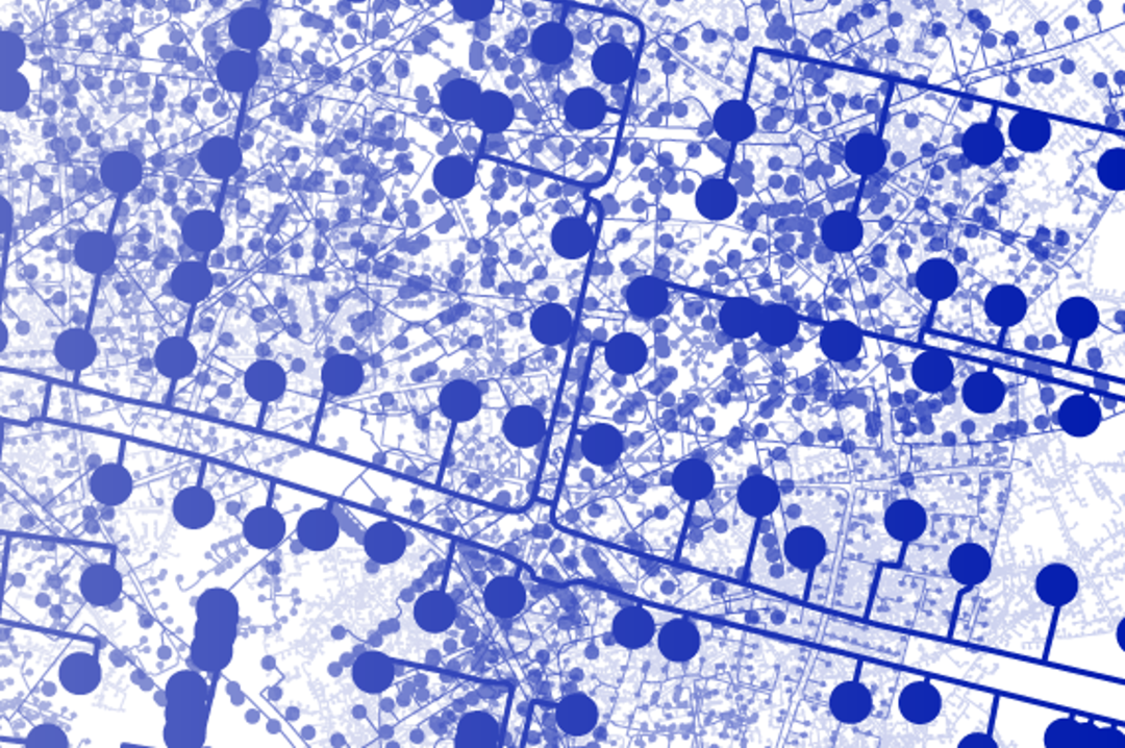
\includegraphics[height=\paperheight]{../Karten/titelbild.pdf}};
		\fill[dnplightblue,path fading=dnpfading] (0, 0) rectangle (\paperwidth, \paperheight);
		\fill[dnpblue] (0, 0) rectangle  (4.7, \paperheight);
		\node[white,anchor=west] at (.2, 7) {\textbf{Ergebnisse}};
		\node[white,anchor=west] at (.2, 6.6) {\Ort};
		\node[white,anchor=west,text width=4.3cm] at (.2, 5) {\scriptsize Adresscheck und Trenches auf Basis von Bildmaterialien};
		\node[white,anchor=south west] at (.2, .2) {\tiny \Abgabedatum};
		\node[anchor=south east] at (\paperwidth, .1) {
\includegraphics[width=.1\textwidth]{../Bilder/Logo.png}};
	\end{tikzpicture}
\end{frame}
}

\addtocounter{framenumber}{-1} %exclude titlepage from page numbering

\begin{frame}{Struktur und Inhalt der Lieferung \Ort}
	\begin{bulletlist}{5pt}
		\item Ergebnis Adresscheck auf Basis von Bildmaterialien
			\begin{bulletlist}{3pt}
				\item[$\bullet$] Übersicht über Anzahl der Adressen und Einheiten
				\item[$\bullet$] Analysebeispiel und Besonderheit, jeweils mit Bild
				\item[$\bullet$] Aufschlüsselung nach Anzahl der Einheiten
			\end{bulletlist}
		\item Ergebnis Trenches auf Basis von Bildmaterialen
		\begin{bulletlist}{3pt}
			\item[$\bullet$] Übersicht konkrete Baumeter inkl. Oberflächenaufteilung und Sonderpositionen
			\item[$\bullet$] Analysebeispiel, typische Oberfläche und Besonderheit jeweils mit Bild
			\item[$\bullet$] Verteilung Trenches mit Handschachtung, Trenches im Straßenkörper, \\ Trenches auf Privatweg
		\end{bulletlist}
		\item Vollständige Plandaten
		\begin{bulletlist}{3pt}
			\item[$\bullet$] Adresskulisse, Trenches inkl. Oberfläche, Fotopunkte, \\ Besonderheiten (GeoPackage)
			\item[$\bullet$] Adressliste, Zusammenfassung Adresscheck, \\ Zusammenfassung Trenches (Excel)
		\end{bulletlist}
	\end{bulletlist}
\end{frame}

\begin{mapframe}{Ergebnis Adresscheck -- Übersicht}{../Karten/adresscheck.pdf}{.5\linewidth}
	\centering
	\resizebox{\textwidth}{!}{\adressStatistik}
\end{mapframe}

\begin{mapframe}{Ergebnis Adresscheck -- Analysebeispiel}{../Karten/adresscheck.pdf}{.55\textwidth}
	\centering
	\tikz[remember picture]{
		\node[inner sep=0] (adresseAnalysebeispiel) at (0,0) {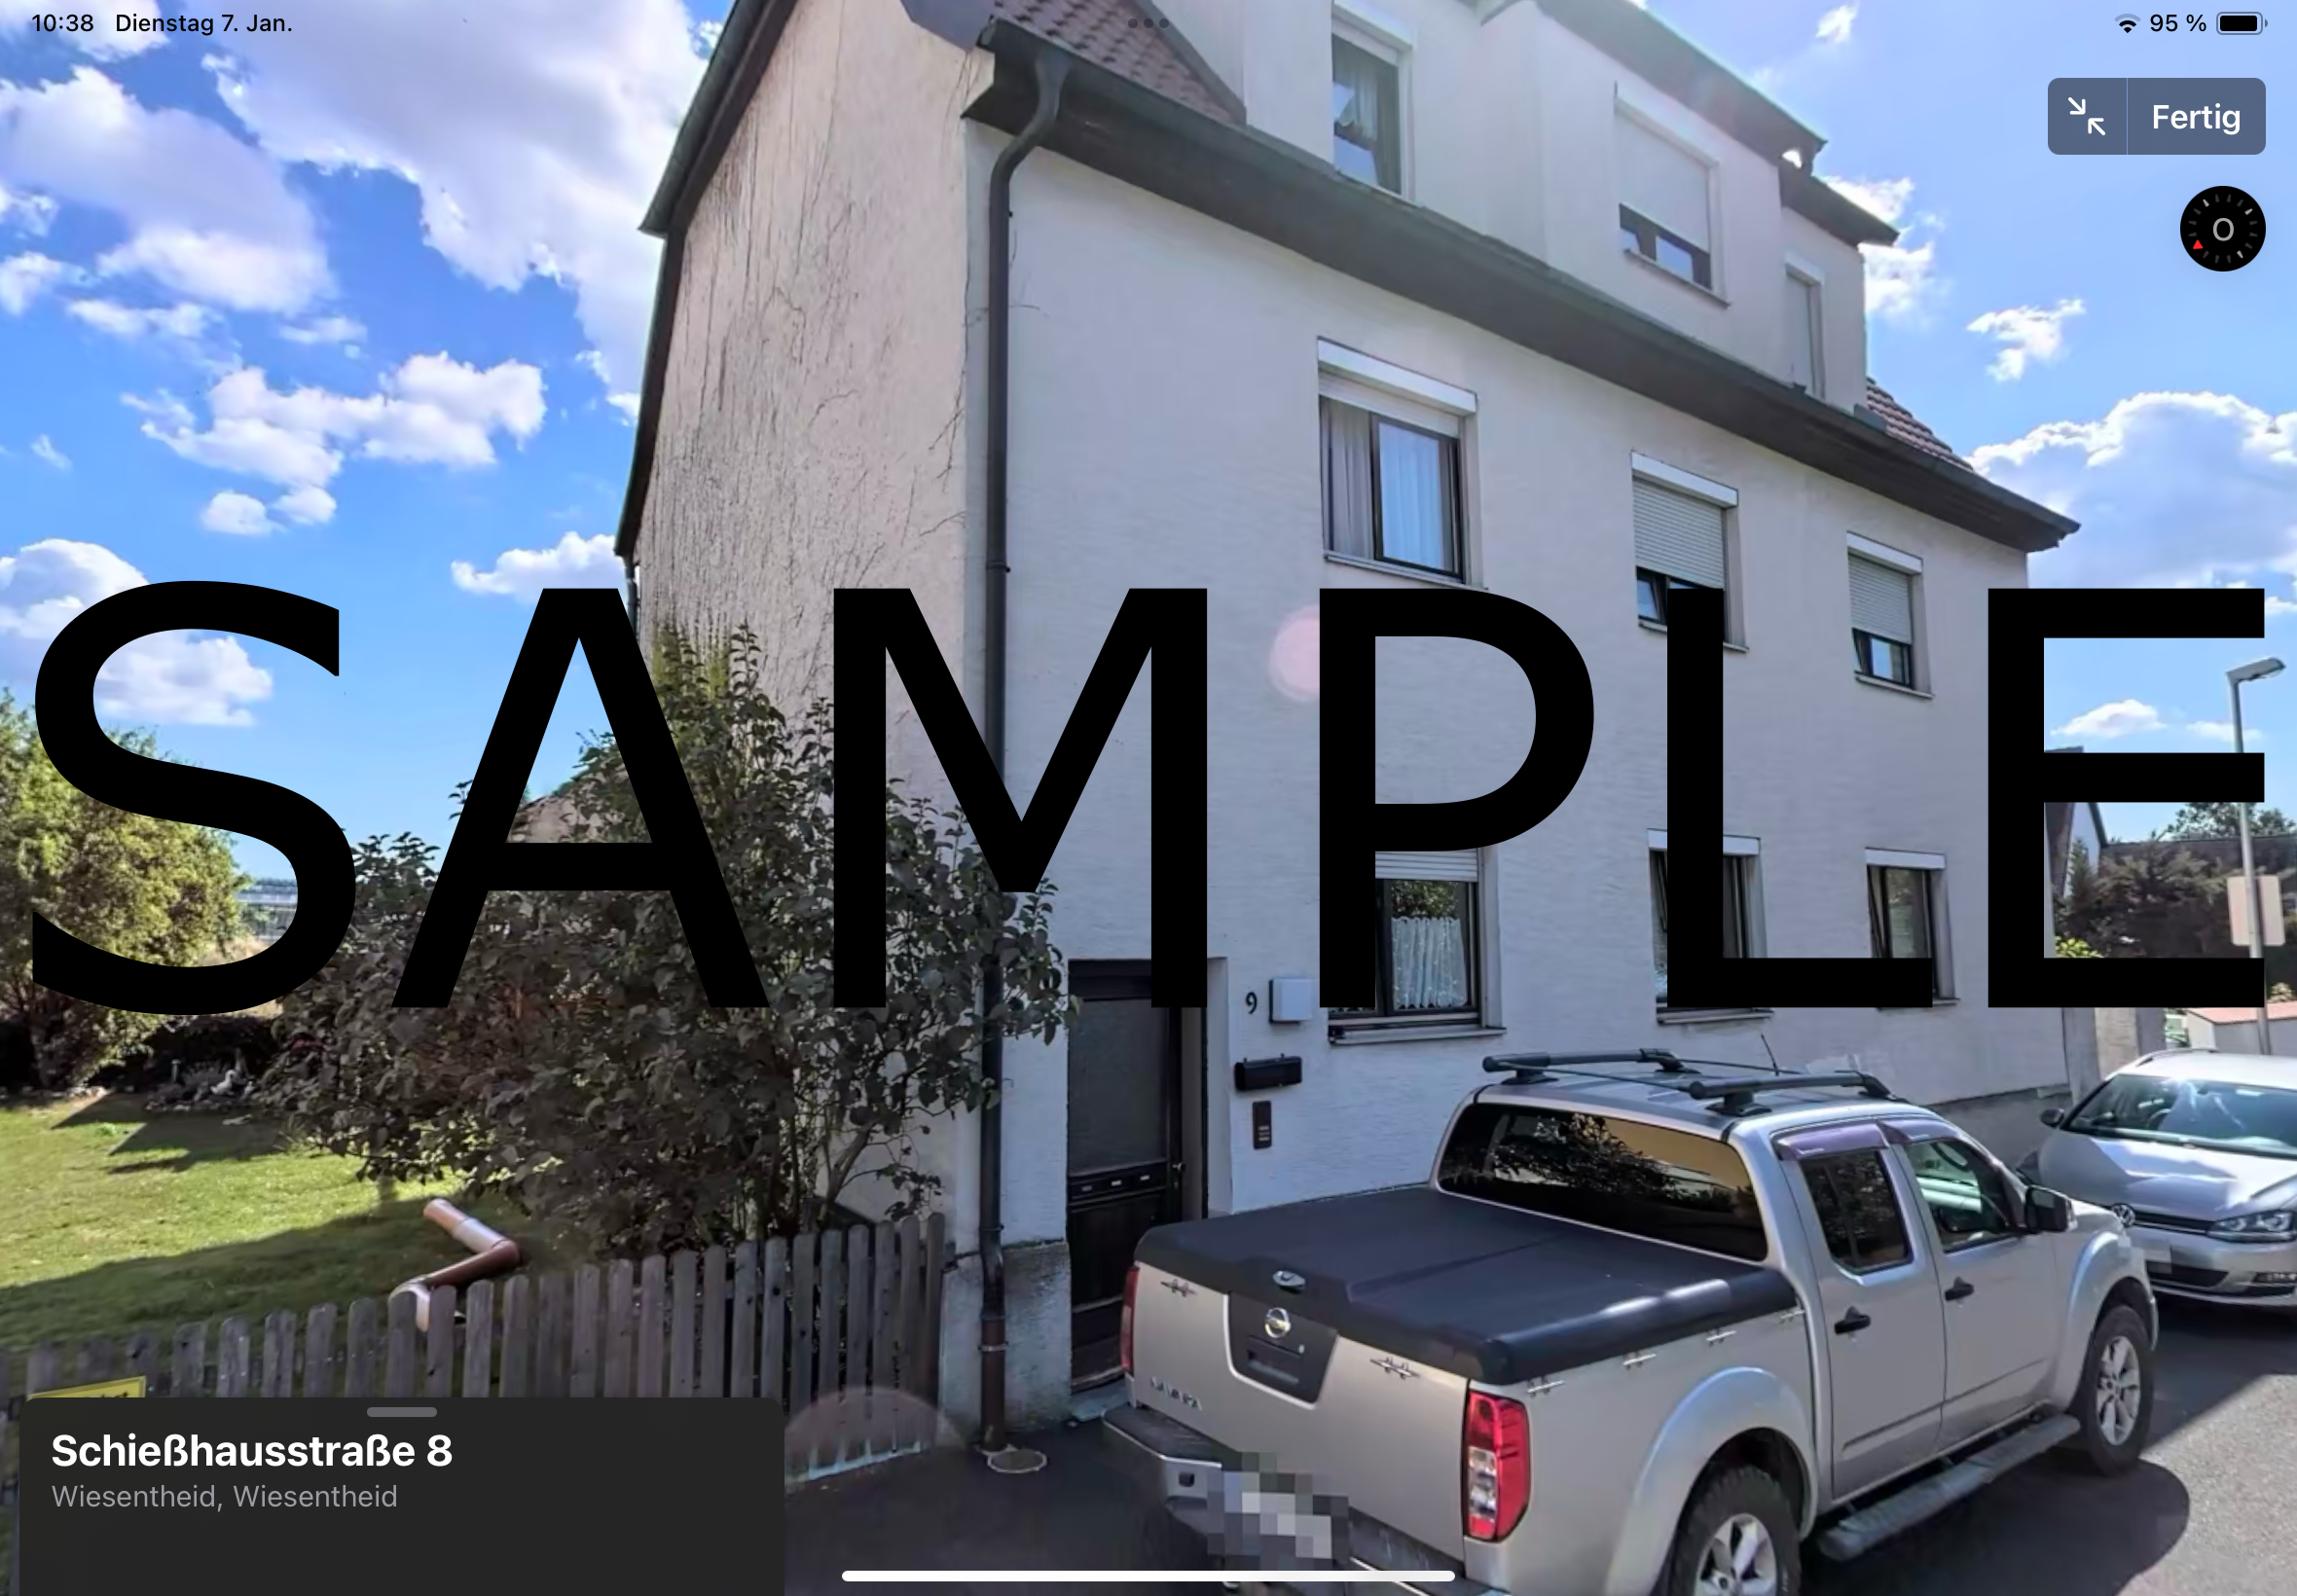
\includegraphics[width=5.7cm]{../Bilder/analysebeispiel-adressen.png}};
	} \\
	\tiny \adresseAnalysebeispiel \\
	\vspace{.2cm}
	\resizebox{5.81cm}{!}{
	\begin{tblr}[expand=\einheitenAnalysebeispiel]{colspec={llll},row{1}={bg=dnpblue,fg=white,font=\bfseries},row{2}={bg=dnplightblue,fg=black}}
		& Grunddaten \Kunde & Adresscheck DNP & Differenz \\
		Anzahl Einheiten & \einheitenAnalysebeispiel
	\end{tblr}
	}
	\zoomtriangle{1}{adresseAnalysebeispiel}{\pointofinterestoneX}{\pointofinterestoneY}
\end{mapframe}

\begin{mapframe}{Ergebnis Adresscheck -- Besonderheit}{../Karten/adresscheck.pdf}{.55\textwidth}
	\centering
	\tikz[remember picture]{
		\node[inner sep=0] (adresseBesonderheit) at (0,0) {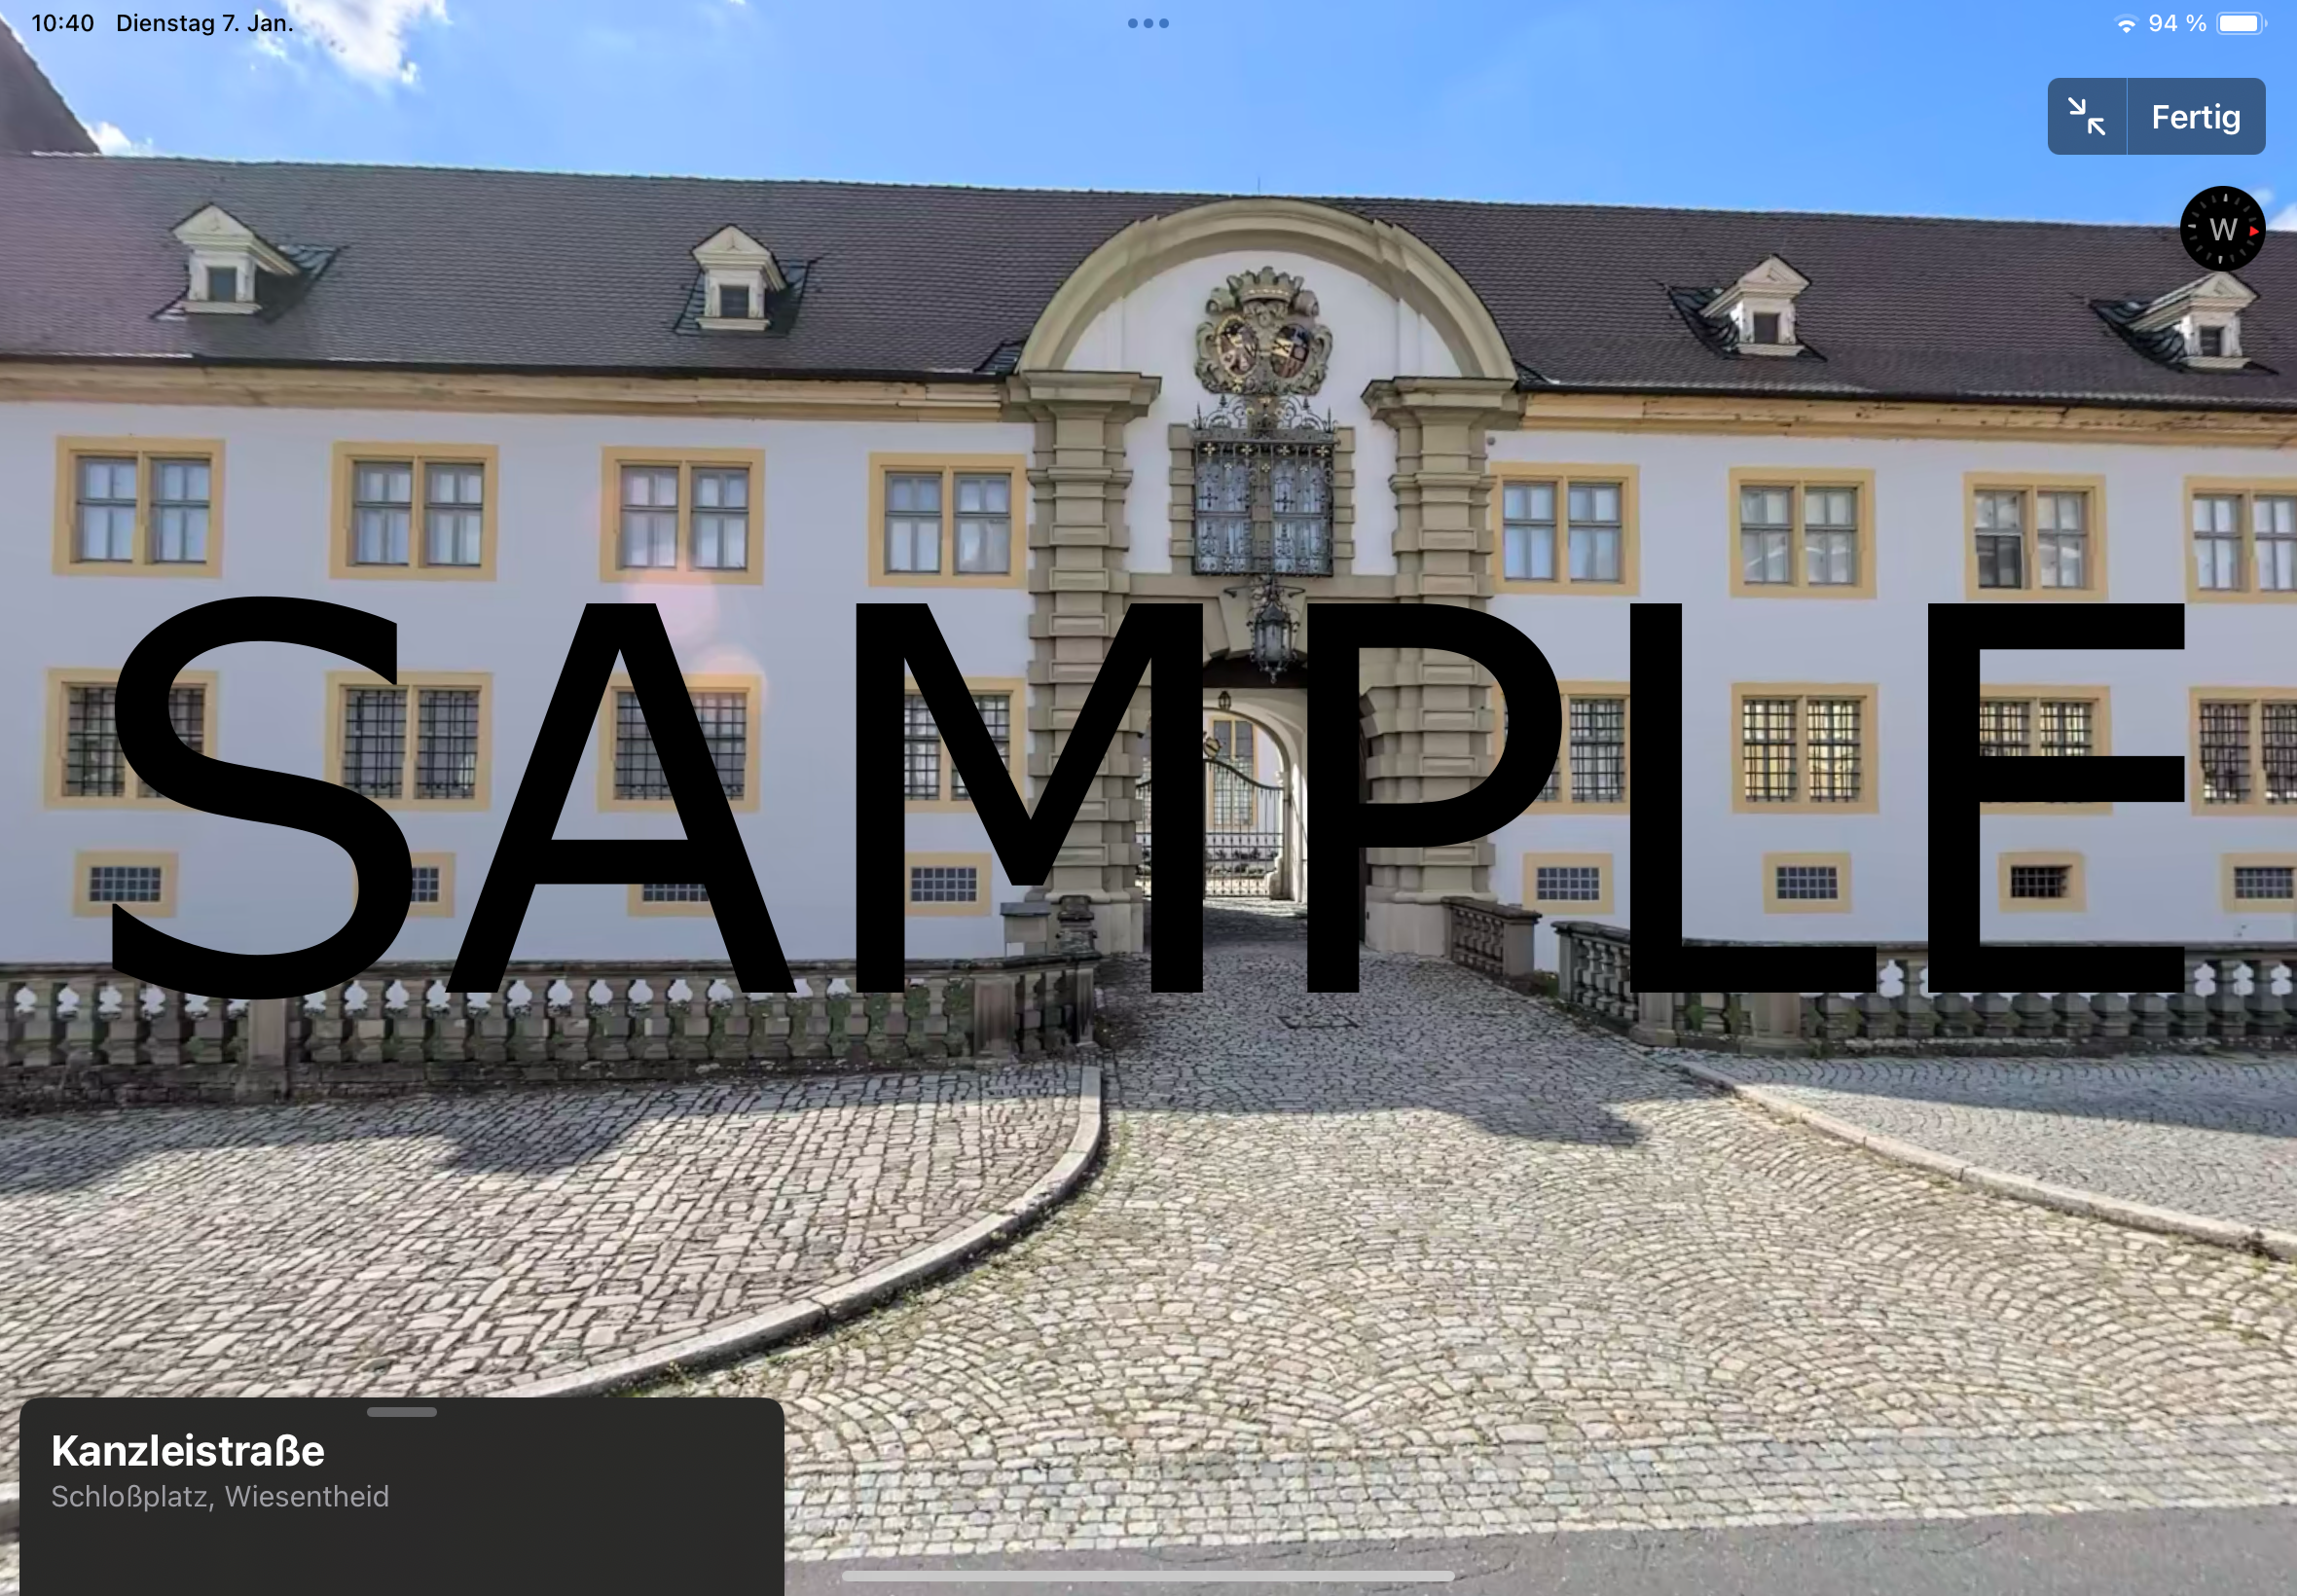
\includegraphics[width=5.7cm]{../Bilder/besonderheit-adressen.png}};
	} \\
	\tiny \besonderheitAdressen
	\zoomtriangle{2}{adresseBesonderheit}{\pointofinteresttwoX}{\pointofinteresttwoY}
\end{mapframe}

\begin{mapframe}{Ergebnis Adresscheck -- Aufschlüsselung nach Anzahl Einheiten}{../Karten/hp-verteilung.pdf}{.55\textwidth}
	\begin{bulletlist}{3pt}
		\item[\colordot{addressgreen}] Ein- und Zweifamilienhäuser
		\item[\colordot{addressorange}] Mehrfamilienhäuser
		\item[\colordot{addressblue}] Hochhäuser ($\geqslant$ 12 Einheiten)
	\end{bulletlist}
\end{mapframe}

\begin{mapframe}{Ergebnis Trenches -- Übersicht}{../Karten/trenches.pdf}{.5\linewidth}
	\centering
	\resizebox{\textwidth}{!}{
		\trenchStatistik
	} \\\vspace{.5cm}
	\hfill\begin{minipage}{.98\textwidth} \tiny
	\textbf{Sonderquerungen}: \sonderquerungen
	\end{minipage}\hfill
\end{mapframe}

\begin{mapframe}{Ergebnis Trenches -- Analysebeispiel}{../Karten/trenches.pdf}{.6\textwidth}
	\centering
	\tikz[remember picture]{
		\node[inner sep=0] (trenchesAnalysebeispiel) at (0,0) {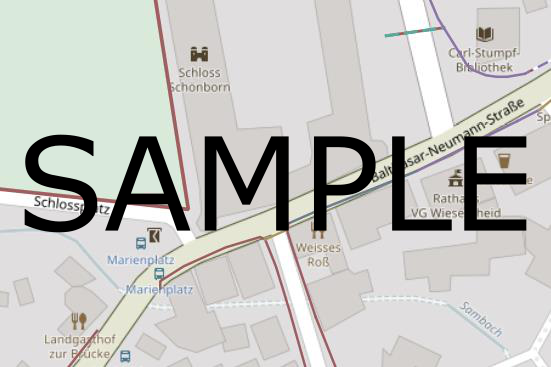
\includegraphics[width=\linewidth]{../Bilder/analysebeispiel-trenches.png}};
	} \\
	\tiny Konkrete Baumeter auf Basis der Adresskulisse
	\zoomtriangle{3}{trenchesAnalysebeispiel}{\pointofinterestthreeX}{\pointofinterestthreeY}
\end{mapframe}

\begin{mapframe}{Ergebnis Trenches -- typische Oberfläche}{../Karten/trenches.pdf}{.6\textwidth}
	\centering
	\tikz[remember picture]{
		\node[inner sep=0] (trenchesTypisch) at (0,0) {\includegraphics[width=\linewidth]{../Bilder/typische-oberflaeche.png}};
	} \\
	\tiny \typischeOberflaeche
	\zoomtriangle{4}{trenchesTypisch}{\pointofinterestfourX}{\pointofinterestfourY}
\end{mapframe}

\begin{mapframe}{Ergebnis Trenches -- Besonderheit}{../Karten/trenches.pdf}{.6\textwidth}
	\centering
	\tikz[remember picture]{
		\node[inner sep=0] (trenchesBesonderheit) at (0,0) {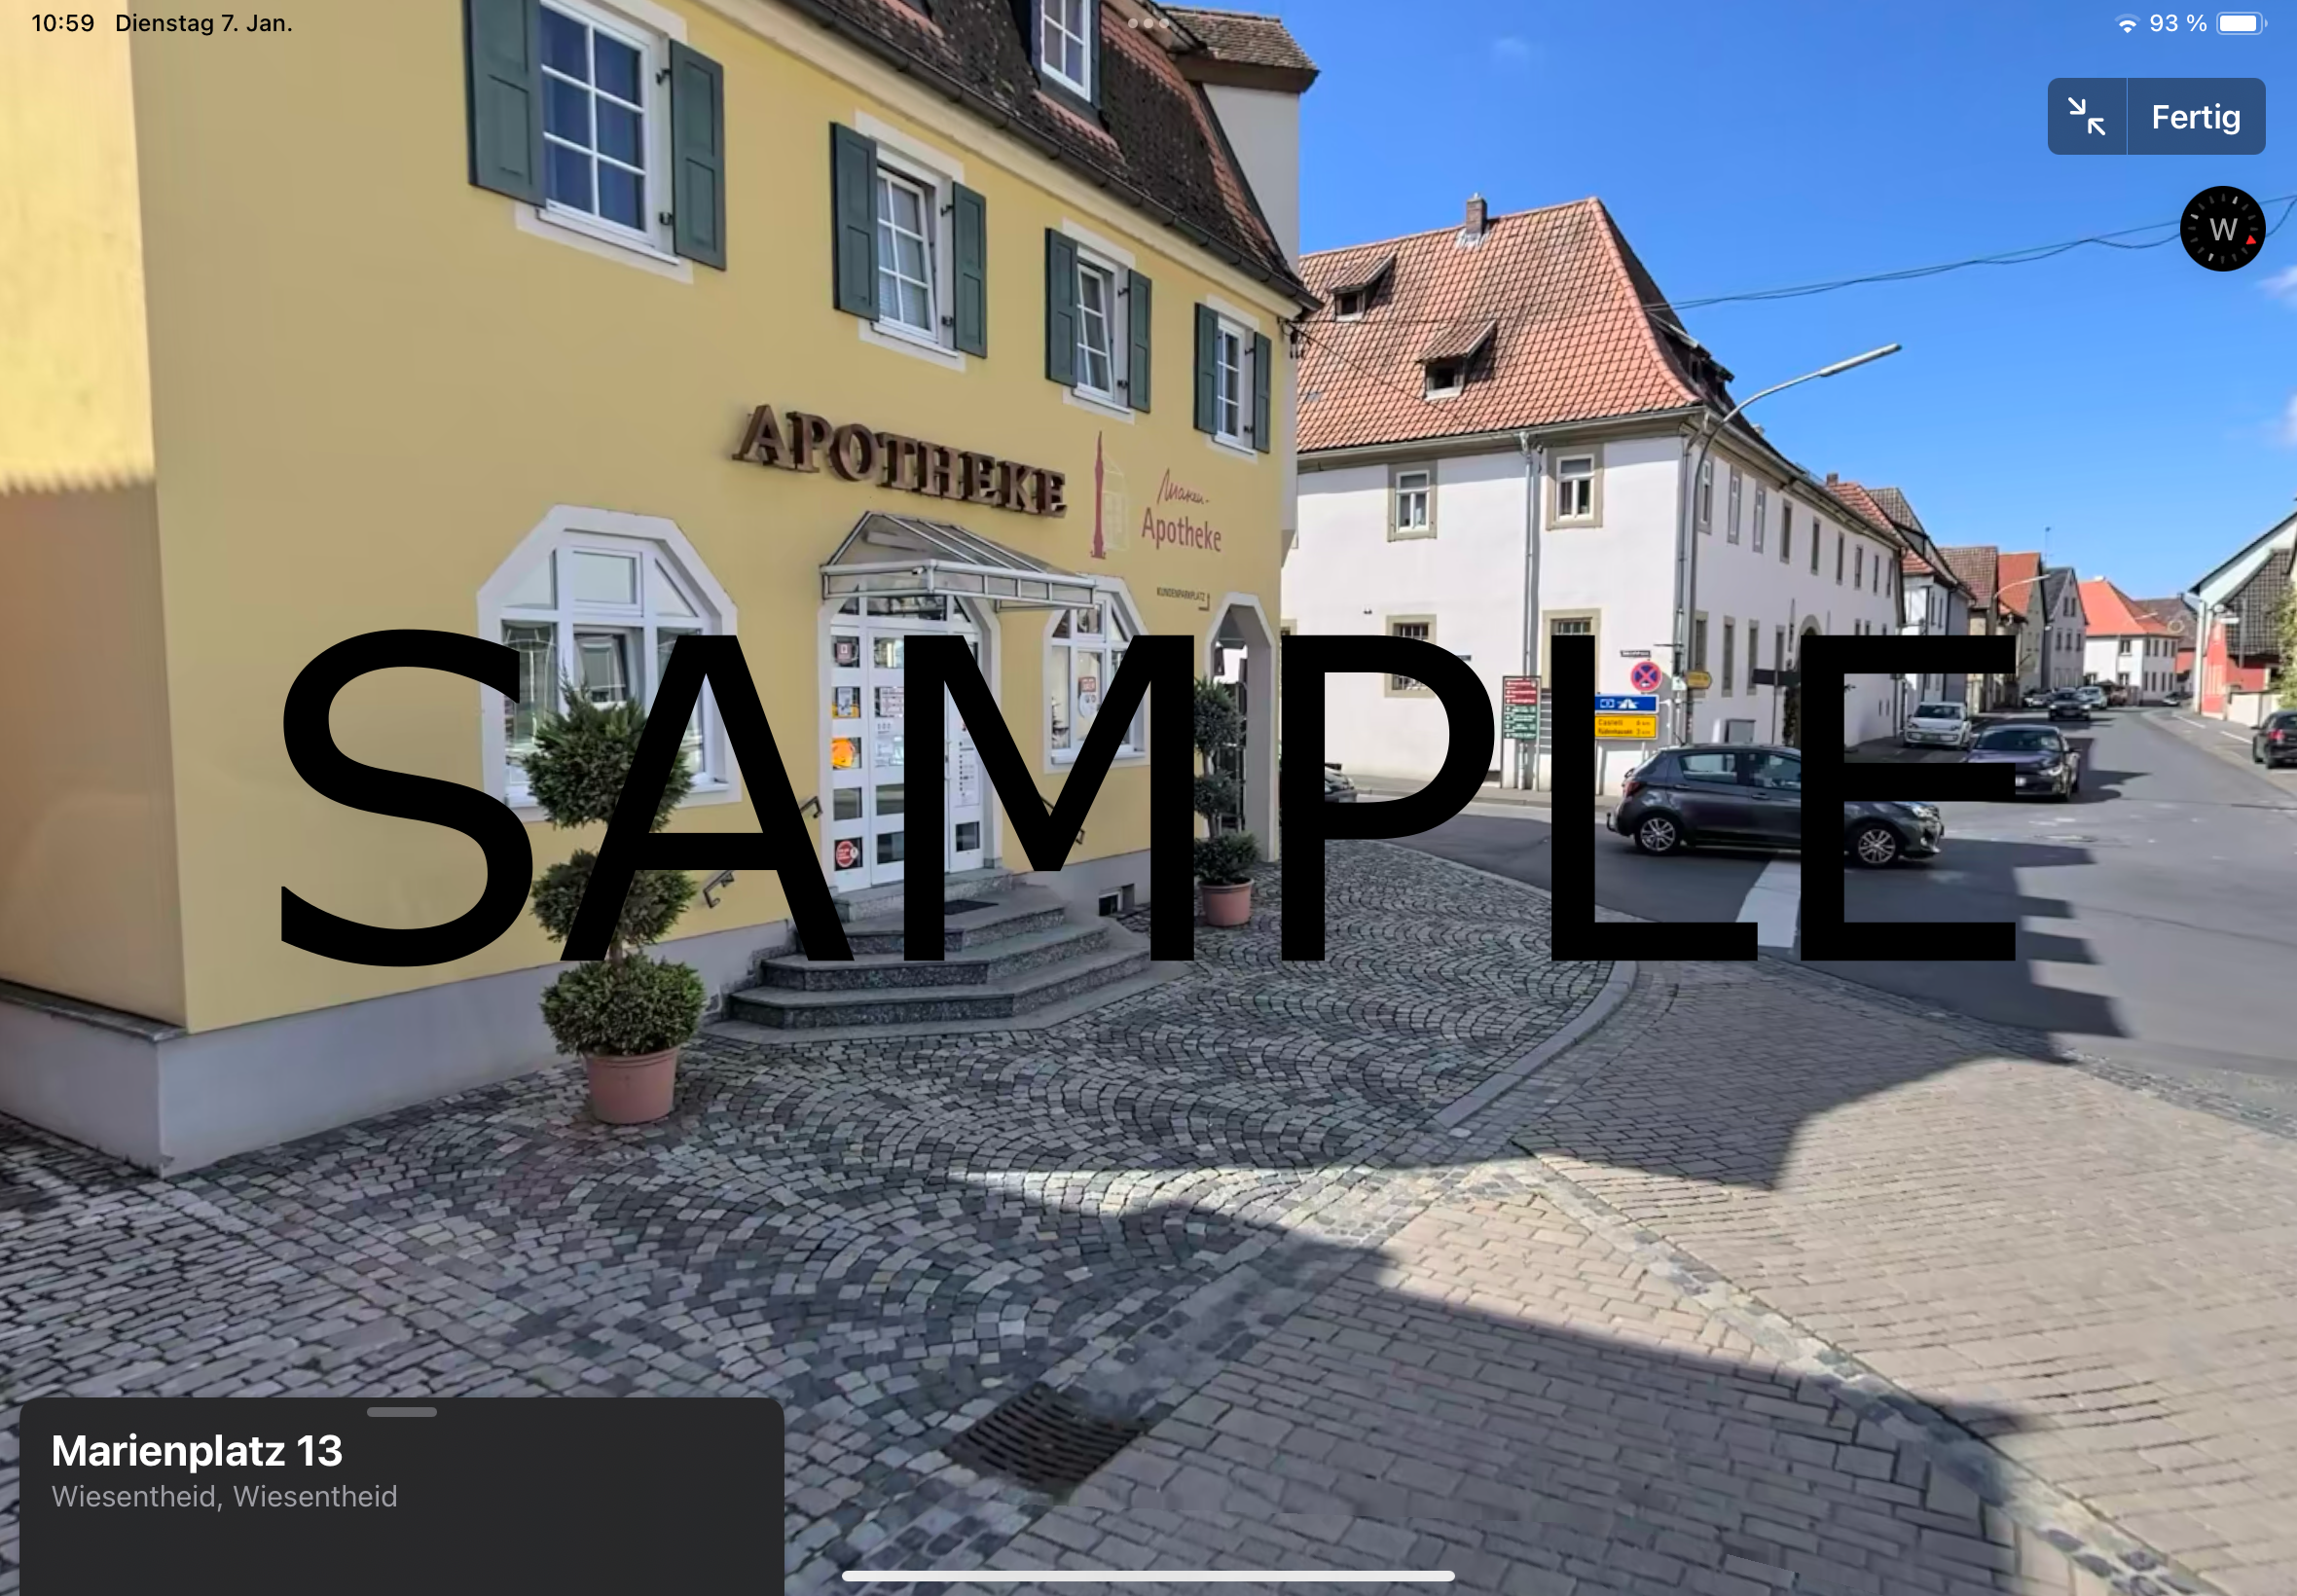
\includegraphics[width=\linewidth]{../Bilder/besonderheit-trenches.png}};
	} \\
	\tiny \besonderheitTrenches
	\zoomtriangle{5}{trenchesBesonderheit}{\pointofinterestfiveX}{\pointofinterestfiveY}
\end{mapframe}

\begin{mapframe}{Ergebnis Trenches -- Sonderquerung}{../Karten/trenches.pdf}{.6\textwidth}
	\centering
	\tikz[remember picture]{
		\node[inner sep=0] (trenchesSonderquerung) at (0,0) {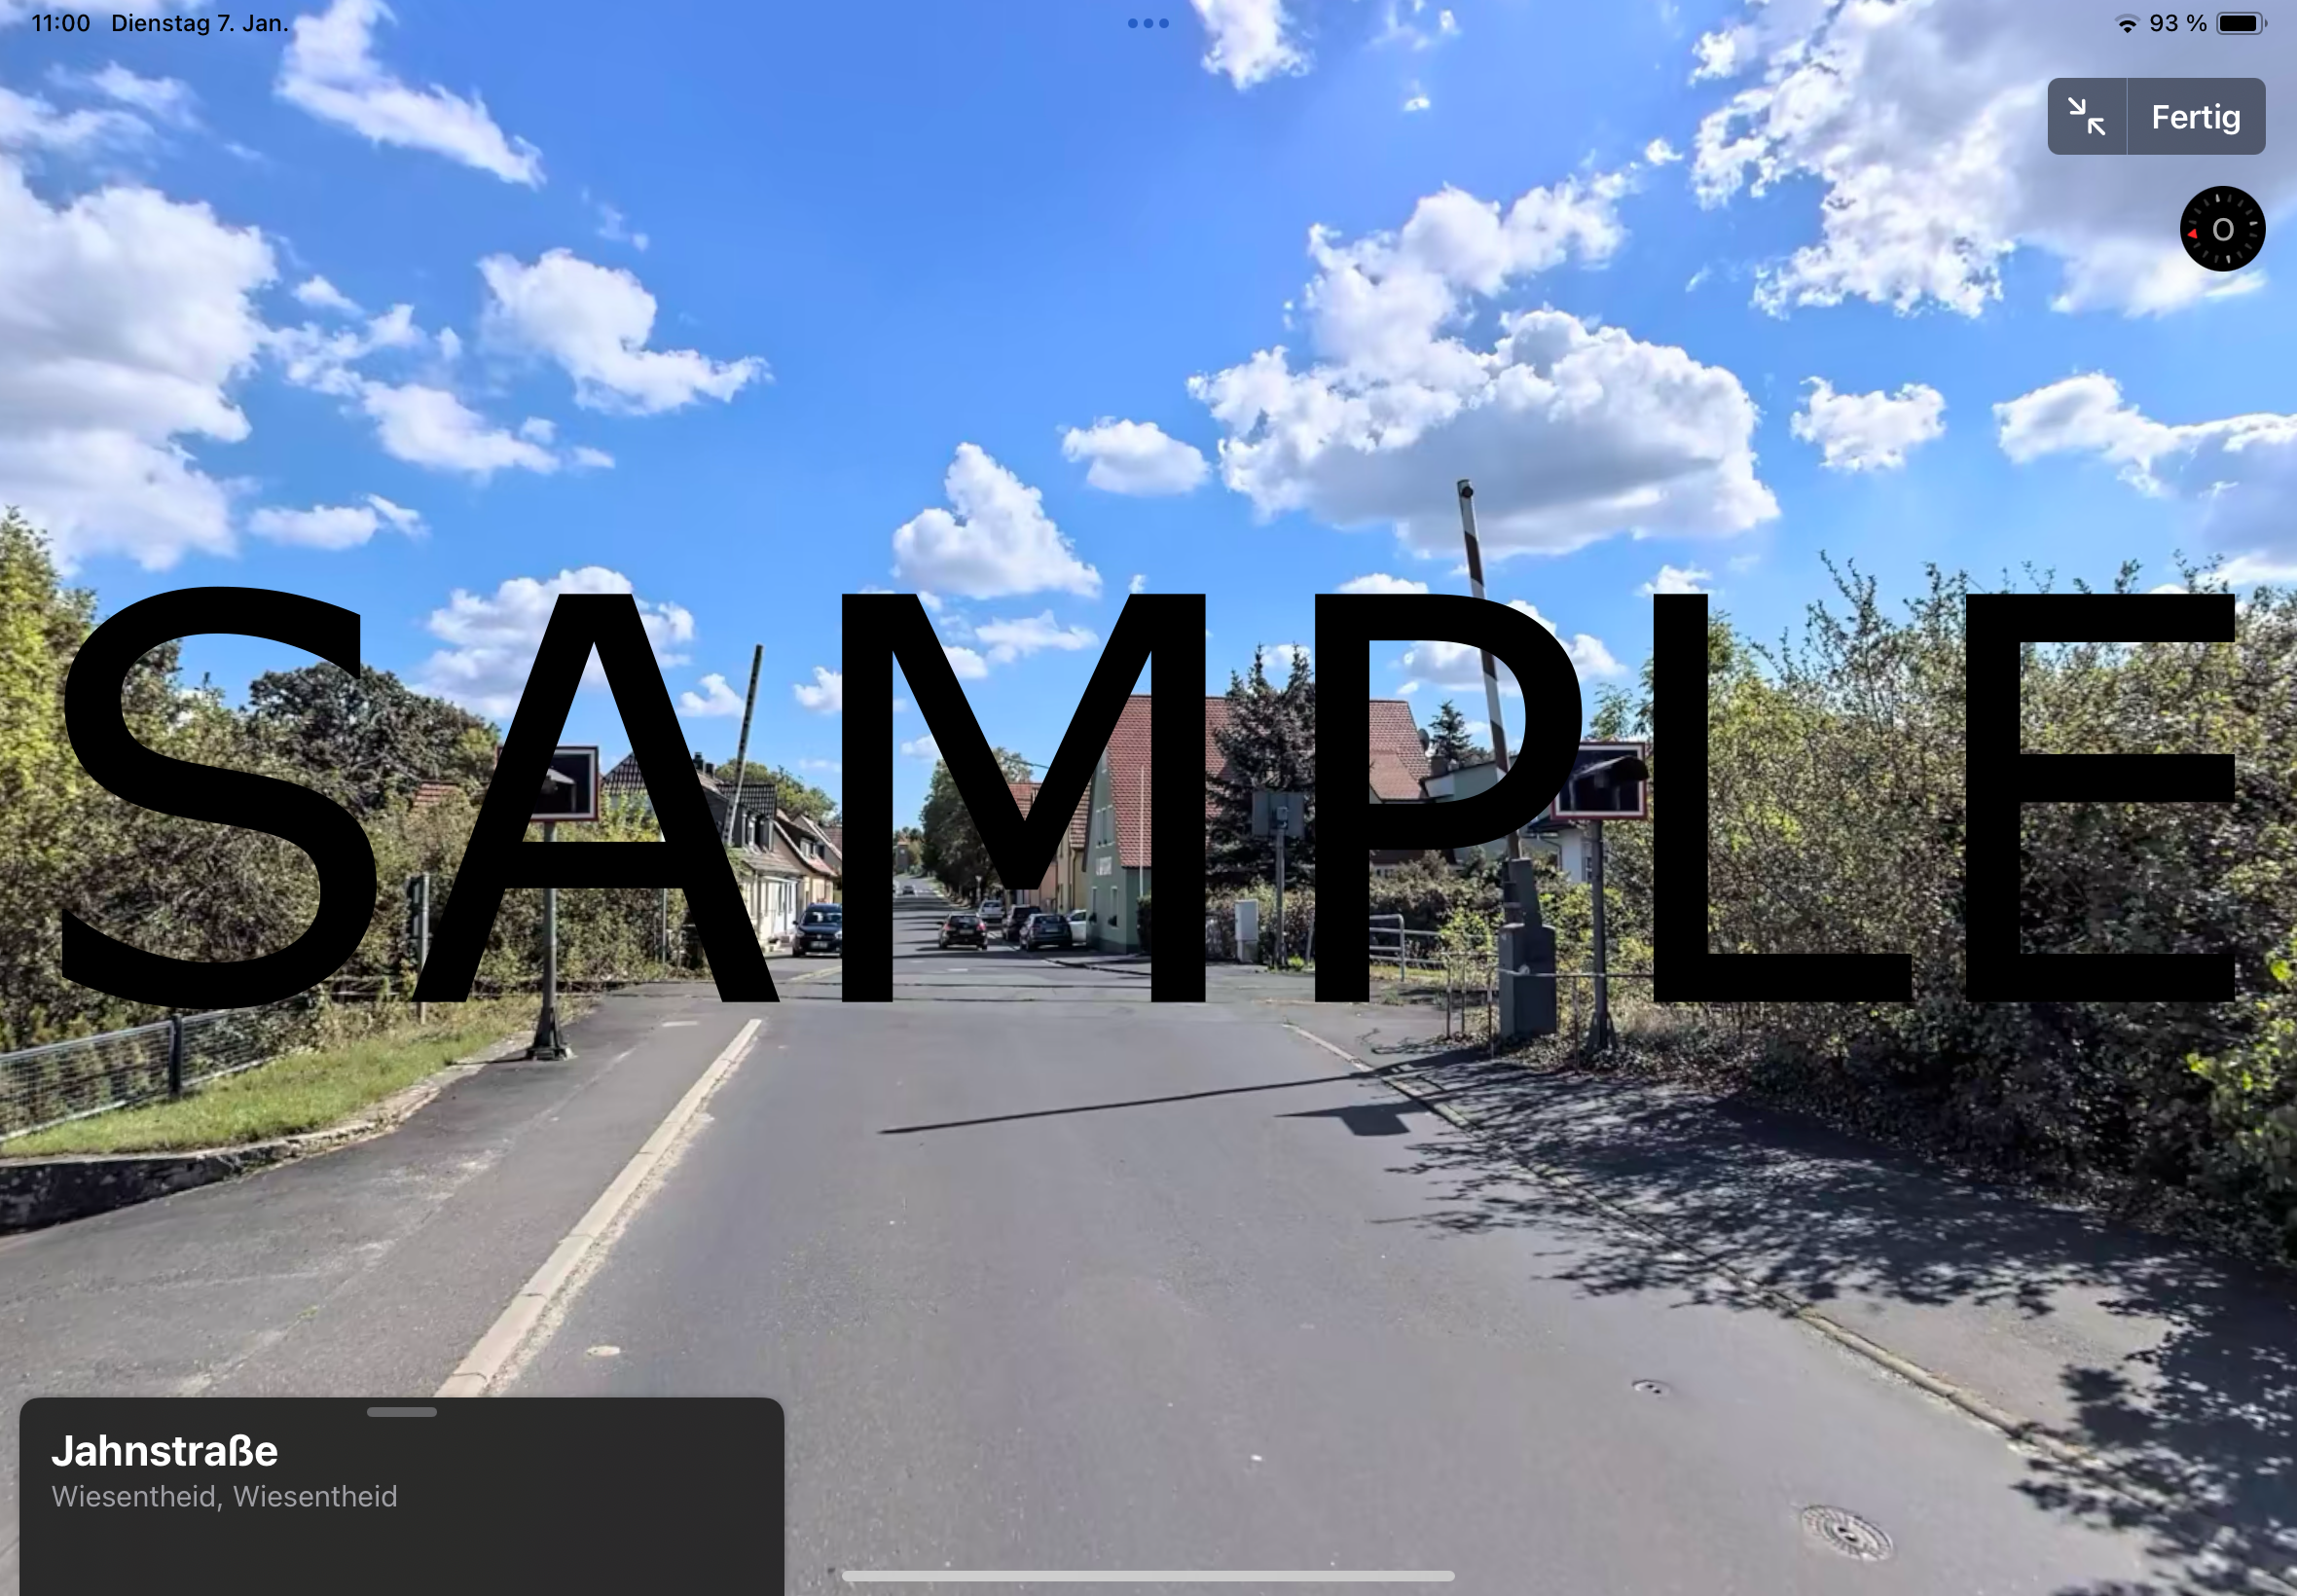
\includegraphics[width=\linewidth]{../Bilder/sonderquerung.png}};
	} \\
	\tiny \sonderquerung
	\zoomtriangle{6}{trenchesSonderquerung}{\pointofinterestsixX}{\pointofinterestsixY}
\end{mapframe}

\begin{mapframe}{Ergebnis Trenches -- Verteilung Handschachtung}{../Karten/trenches-handschachtung.pdf}{.6\textwidth}
	\begin{itemize}
		\item[\colorrule{trenchgreen}] Trench \textbf{mit} Handschachtung
		\item[\colorrule{trenchblack}] Trench \textbf{ohne} Handschachtung
	\end{itemize}
\end{mapframe}

\begin{mapframe}{Ergebnis Trenches -- Verteilung Trench im Straßenkörper}{../Karten/trenches-strassenkoerper.pdf}{.6\textwidth}
	\begin{itemize}
		\item[\colorrule{trenchred}] Trench im \textbf{Straßenkörper}
		\item[\colorrule{trenchblack}] Trench im \textbf{Gehweg}
	\end{itemize}
\end{mapframe}

\begin{mapframe}{Ergebnis Trenches -- Verteilung Trench auf Privatweg}{../Karten/trenches-privatweg.pdf}{.6\textwidth}
	\begin{itemize}
		\item[\colorrule{trenchblue}] Trench auf \textbf{Privatweg}
		\item[\colorrule{trenchblack}] Trench auf \textbf{öffentlichem Grund}
	\end{itemize}
\end{mapframe}


\end{document}